\documentclass[xcolor={dvipsnames}]{beamer}
%\usepackage[utf8]{inputenc}
\usetheme{Madrid}
%\usetheme{Malmoe}
\usecolortheme{beaver}
%\usecolortheme{rose}

%-------------------------------------------------------------------------------
%          -Packages nécessaires pour écrire en Français et en UTF8-
%-------------------------------------------------------------------------------
\usepackage[utf8]{inputenc}
\usepackage[frenchb]{babel}
\usepackage[T1]{fontenc}
\usepackage{lmodern}
\usepackage{textcomp}

%-------------------------------------------------------------------------------

%-------------------------------------------------------------------------------
%                          -Outils de mise en forme-
%-------------------------------------------------------------------------------
\usepackage{hyperref}
\hypersetup{pdfstartview=XYZ}
\usepackage{enumerate}
\usepackage{graphicx}
%\usepackage{multicol}
%\usepackage{tabularx}

%\usepackage{anysize} %%pour pouvoir mettre les marges qu'on veut
%\marginsize{2.5cm}{2.5cm}{2.5cm}{2.5cm}

\usepackage{indentfirst} %%pour que les premier paragraphes soient aussi indentés
\usepackage{verbatim}
%\usepackage[table]{xcolor}  
%\usepackage{multirow}
\usepackage{ulem}
%-------------------------------------------------------------------------------


%-------------------------------------------------------------------------------
%                  -Nécessaires pour écrire des mathématiques-
%-------------------------------------------------------------------------------
\usepackage{amsfonts}
\usepackage{amssymb}
\usepackage{amsmath}
\usepackage{amsthm}
\usepackage{tikz}
\usepackage{xlop}
\usepackage[output-decimal-marker={,}]{siunitx}
%-------------------------------------------------------------------------------


%-------------------------------------------------------------------------------
%                    - Mise en forme 
%-------------------------------------------------------------------------------

\newcommand{\bu}[1]{\underline{\textbf{#1}}}


\usepackage{ifthen}


\newcommand{\ifTrue}[2]{\ifthenelse{\equal{#1}{true}}{#2}{$\qquad \qquad$}}

\newcommand{\kword}[1]{\textcolor{red}{\underline{#1}}}


%-------------------------------------------------------------------------------



%-------------------------------------------------------------------------------
%                    - Racourcis d'écriture -
%-------------------------------------------------------------------------------

% Angles orientés (couples de vecteurs)
\newcommand{\aopp}[2]{(\vec{#1}, \vec{#2})} %Les deuc vecteurs sont positifs
\newcommand{\aopn}[2]{(\vec{#1}, -\vec{#2})} %Le second vecteur est négatif
\newcommand{\aonp}[2]{(-\vec{#1}, \vec{#2})} %Le premier vecteur est négatif
\newcommand{\aonn}[2]{(-\vec{#1}, -\vec{#2})} %Les deux vecteurs sont négatifs

%Ensembles mathématiques
\newcommand{\naturels}{\mathbb{N}} %Nombres naturels
\newcommand{\relatifs}{\mathbb{Z}} %Nombres relatifs
\newcommand{\rationnels}{\mathbb{Q}} %Nombres rationnels
\newcommand{\reels}{\mathbb{R}} %Nombres réels
\newcommand{\complexes}{\mathbb{C}} %Nombres complexes


%Intégration des parenthèses aux cosinus
\newcommand{\cosP}[1]{\cos\left(#1\right)}
\newcommand{\sinP}[1]{\sin\left(#1\right)}

%Fractions
\newcommand{\myfrac}[2]{{\LARGE $\frac{#1}{#2}$}}

%Vocabulaire courrant
\newcommand{\cad}{c'est-à-dire}

%Droites
\newcommand{\dte}[1]{droite $(#1)$}
\newcommand{\fig}[1]{figure $#1$}
\newcommand{\sym}{symétrique}
\newcommand{\syms}{symétriques}
\newcommand{\asym}{axe de symétrie}
\newcommand{\asyms}{axes de symétrie}
\newcommand{\seg}[1]{$[#1]$}
\newcommand{\monAngle}[1]{$\widehat{#1}$}
\newcommand{\bissec}{bissectrice}
\newcommand{\mediat}{médiatrice}
\newcommand{\ddte}[1]{$[#1)$}

%Figures
\newcommand{\para}{parallélogramme}
\newcommand{\paras}{parallélogrammes}
\newcommand{\myquad}{quadrilatère}
\newcommand{\myquads}{quadrilatères}
\newcommand{\co}{côtés opposés}
\newcommand{\diag}{diagonale}
\newcommand{\diags}{diagonales}
\newcommand{\supp}{supplémentaires}
\newcommand{\car}{carré}
\newcommand{\cars}{carrés}
\newcommand{\rect}{rectangle}
\newcommand{\rects}{rectangles}
\newcommand{\los}{losange}
\newcommand{\loss}{losanges}


%----------------------------------------------------


\usepackage{../../../../pas-math}
\usepackage{../../../../moncours_beamer}

\usepackage{amssymb,amsmath}


\newcommand{\myitem}{\item[\textbullet]}

\graphicspath{{../img/}}

\title{Séquence 1 : Calculs et priorités}
%\author{O. FINOT}\institute{Collège S$^t$ Bernard}

%
\AtBeginSection[]
{
	\begin{frame}
		\frametitle{}
		\tableofcontents[currentsection, hideallsubsections]
	\end{frame} 

}
%
%
%\AtBeginSubsection[]
%{
%	\begin{frame}
%		\frametitle{Sommaire}
%		\tableofcontents[currentsection, currentsubsection]
%	\end{frame} 
%}

\begin{document}



\begin{frame}
  \titlepage 
\end{frame}


	

\begin{frame}
	\begin{block}{Objectifs}
		\begin{itemize}
			\item Revoir et appliquer les priorité des opérations;
			\item Calculer une expression avec et sans parenthèses;
			\item Connaître la structure et le vocabulaire d'une expression numérique.		
			
			
		\end{itemize}
	\end{block}
		
		
	\begin{block}{Compétence}
		\textbf{Calculer} : calculer avec des nombres rationnels, de manière exacte  ou approchée, en combinant  de  façon  appropriée  le  calcul  mental,  le  calcul  posé  et  le  calcul instrumenté (calculatrice ou logiciel)
	\end{block}
\end{frame}


\section{Priorités des opérations}


\begin{frame}{}
	\begin{alertblock}{Propriété}
		Dans une suite d'additions ou de multiplications, l'ordre des calculs n'a pas d'importance.
	\end{alertblock}


	\begin{exampleblock}{Exemples}
		\begin{itemize}
			\item $2 + \num{3.4} + 8 + \num{6.6} + 5 = $ \vspace*{2cm}
			
			
			\item $\num{2.5} \times 5 \times 2 = $ \vspace*{1cm}
		\end{itemize}
	\end{exampleblock}
\end{frame}


\begin{frame}{}
	\begin{alertblock}{Propriété}
		Dans une suite de calculs qui contient uniquement des additions et des soustractions on effectue les calculs dans l'ordre d'écriture (de gauche à droite).
	\end{alertblock}
	
	
	\begin{exampleblock}{Exemples}
		\begin{itemize}
			\item $2 + 8 - 3 + 7 - 5 =$ \vspace*{2cm}
			
			
			\item $ \num{2.5} \times 10 \div 5 \times 2 = $\vspace*{1cm}
		\end{itemize}
	\end{exampleblock}
\end{frame}


\begin{frame}{}
	\begin{alertblock}{Propriété}
		Dans une suite de calculs sans parenthèses on effectue les multiplications et les divisions avant les additions et les soustractions
	\end{alertblock}
	
	
	\begin{exampleblock}{Exemples}
		\begin{itemize}
			\item $4 + 5 \times 3 = $ \vspace*{2cm}
			
			
			\item $ 3 + 8 \div 2 - 2 \times 2 = $\vspace*{1cm}
		\end{itemize}
	\end{exampleblock}
\end{frame}

\begin{frame}{}
	\begin{alertblock}{Propriété}
		Dans une suite de calculs on effectue d'abord les calculs entre parenthèses. On commence toujours par les parenthèses les plus à l'intérieur.
	\end{alertblock}
	
	
	\begin{exampleblock}{Exemples}
		\begin{itemize}
			\item $(4 + 5) \times 3 =$  \vspace*{2cm}
			
			
			\item $ (3 + 8 \div (6 - 2)) \times 2 = $ \vspace*{1cm}
		\end{itemize}
	\end{exampleblock}
\end{frame}

%\begin{frame}
%	\begin{exampleblock}{Exemples}
%		\begin{itemize}
%			\myitem Je calcule l'expression $A= 20 - 2 \times 3 + 12 \div 6$ :\pause
%			
%			\vspace*{-0.5cm}
%			
%			\begin{eqnarray*}
%				A &=& 20 - 2 \times 3 + 12 \div 6 \\ \pause
%				A &=& 20 - 6 + 12 \div 6 \text{ (je commence par la multiplication) }\\ \pause
%				A &=& 20 - 6 + 2 \text{ (ensuite la division)} \\ \pause
%				A &=& 14 + 2 \text{ (puis le reste des opérations de gauche à droite)}\\ \pause
%				A &=& 16 \pause
%			\end{eqnarray*}
%			
%			\myitem Je calcule l'expression $B= 12 + 3 +8$ de trois façons différentes : \pause
%			
%			\vspace*{-0.5cm}
%			\begin{columns}
%				\begin{column}{0.33\textwidth}
%					\begin{eqnarray*}
%						B &=& \underline{12 + 3} + 8 \\
%						B &=& 15 + 8 \\
%						B &=& 23
%					\end{eqnarray*}
%				\end{column}\pause
%				
%				\begin{column}{0.33\textwidth}
%					\begin{eqnarray*}
%						B &=& 12 + \underline{3 + 8} \\
%						B &=& 12 + 11 \\
%						B &=& 23
%					\end{eqnarray*}
%				\end{column}\pause
%				
%				
%				\begin{column}{0.33\textwidth}
%					\begin{eqnarray*}
%						B &=& \underline{12 + 8} + 3 \\
%						B &=& 20 + 3 \\
%						B &=& 23
%					\end{eqnarray*}	
%				\end{column}
%				
%			\end{columns}
%			
%		\end{itemize}
%	\end{exampleblock}
%\end{frame}
%
%\section{Calculer une expression}
%
%
%\begin{frame}
%	\begin{alertblock}{Propriétés}
%		\begin{itemize}
%			\item Dans une expression numérique qui contient des parenthèses, on calcule :
%			\begin{enumerate}
%				\item d'abord les opérations entre parenthèses;\pause
%				\item puis on calcule l'expression sans parenthèses obtenue.\pause
%			\end{enumerate}
%			
%			\item Si l'expression contient des parenthèses imbriquées, on commence par celles qui sont le plus à l'intérieur.
%		\end{itemize}
%	\end{alertblock}
%
%\begin{myex}
%	Je calcule l'expression $C = (3 \times (7 - 3))  + 1$ :\pause
%	
%	\vspace*{-0.5cm}
%	
%	\begin{eqnarray*}
%		C & = & (3  \times   \underbrace{(7-3)})  + 1 \\ \pause %\text{ (on commence par la parenthèse intérieure)} \\
%		C & = & \quad \: \underbrace{(3 \times 4)}+ 1 \\ \pause%\text{ (puis l'autre)} \\
%		C & = & \qquad \underbrace{12  + 1} \\ \pause%\text{ (enfin on calcule le reste de l'expression)}\\
%		C & = & \qquad \quad 13
%	\end{eqnarray*}
%\end{myex}
%\end{frame}
%
\section{Vocabulaire}
\begin{frame}
	\begin{alertblock}{Définition}
		\begin{itemize}
			\item Le résultat d'une \kword{addition} est une \pause \kword{somme}, les nombres utilisés sont \pause des \kword{termes}.\pause
			
			\item Une \kword{différence} est le résultat de la \pause  \kword{soustraction} de deux \kword{termes}.\pause
			
			\item Un \kword{produit} est le résultat de la \pause \kword{multiplication} de deux \kword{facteurs}.\pause
			
			\item Le résultat de la \kword{division} d'un \pause \kword{dividende} par un \kword{diviseur} est un \kword{quotient}.
		\end{itemize}
		
	\end{alertblock}

\end{frame}

\begin{frame}
	
	\begin{exampleblock}{Exemple}
		\begin{center}
			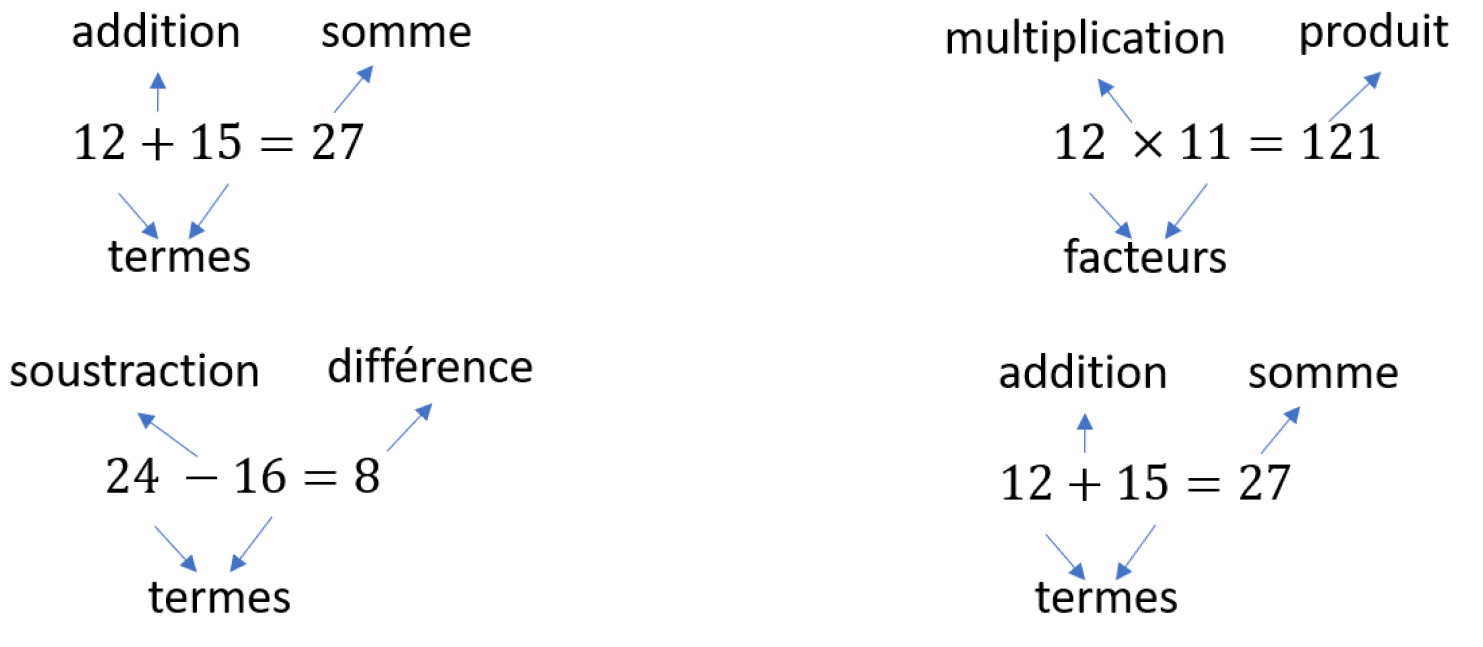
\includegraphics[scale=0.31]{op}
		\end{center}
	\end{exampleblock}
	
\end{frame}


%
\begin{frame}
	\begin{myexs}
		\begin{itemize}
			\item L'expression $5 + 3 \times 4$ est \pause la somme de 5 et du produite de 3 par 4.\pause
			
			\item L'expression $(2 + 3 ) \times 4$ est \pause le produit de la somme de 2 et 3 par 4.\pause
			
					
			\item $(19 - 3) \div (2 \times 4)$ est \pause le quotient de la différence entre  19 et 3 par le produit de 2 par 4.
		\end{itemize}
	\end{myexs}
\end{frame}
\end{document}